\documentclass[letterpaper,twocolumn,10pt]{article}

\usepackage{tikz}
\usepackage{amsmath}
\usepackage{graphicx}
\usepackage{float}
\usepackage{lipsum}
\usepackage{sidecap}
\usepackage{hyperref}
\usepackage{xcolor}

\usepackage{titling}

%\usepackage[left=0.5in,right=0.5in, bottom=0.5in]{geometry}
\setlength{\droptitle}{-0.6in}
\usepackage[margin=0.5in]{geometry}



%-------------------------------------------------------------------------------
\begin{document}
% -------------------------------------------------------------------------------

\date{} % avoid printing of date

\title{Serial-Optimising Chessboard-Pattern Stenciling}

\author{
  {\rm Jan Fecht}\\
  University of Bristol}

\maketitle


% -------------------------------------------------------------------------------
\section*{Introduction}
% -------------------------------------------------------------------------------
The program to be optimised consists of a simple stencil applied on a chessboard-pattern image.
The user can specify the width $nx$ and the height $ny$ of the image and furthermore
the number of times $k$ that the stencil is applied. All of these parameters are passed on the command line to the program, except for $k$ which is passed as $k/2$ (niters) instead.

For comparing and evaluating the effect of
the algorithmic optimisation, the final version of the code was benchmarked
and compared to the final version without the optimisation. The reason for this is
that the optimisation was introduced rather late which makes it hard
to apply the optimisation seperatly onto the original version as a lot of code rewriting
would be necessary.
Memory and Vectorization related optimisations, on the other hand, are introduced in a
progressive manner, starting with the original version.

Measured times were determined by taking the average of 100 runs
on the University's \textit{Blue Crystal 4} supercomputer (\textit{bc4}). The times for
the original version were taken from the official repository
\footnote{\url{https://github.com/UoB-HPC/intro-hpc-stencil/}} instead as running it 100 times would have been infeasible.

The speedup of the final version can be seen in Table~\ref{tab:final}.

\vspace{0.10in}

\textbf{Disclaimer} The optimisations applied were neither introduced
in the order nor grouped together as they are described in this report. Rather, the 
whole optimisation process was iterative because new ideas and adaptions to new
circumstances were necessary. To see the full progression, run \texttt{git log} in the root
of the project directory.

\begin{table}[ht]
	\vspace{-0.2in}
	\caption{Original compared to final version ($k=200$).}
	\begin{tabular}{c c c c}
		 image size & original & final & speedup \\
		 \hline
		1024 x 1024 & 5.908341s   & 0.01626971s & 363.15\\
		4096 x 4096 & 130.196475s & 0.02686471s & 4846.38\\
		8000 x 8000 & 561.118133s & 0.0451399s & 12430.65\\
	\end{tabular}
	\label{tab:final}
	\vspace{-0.3in}
\end{table}

% -------------------------------------------------------------------------------
\section*{Algorithm}
% -------------------------------------------------------------------------------
The chessboard pattern contains a high degree of symmetry and by applying the stencil code
to all points the original code performs plenty of redundant computations.
The number of floating point operations lies in $\Theta(nx * ny * k)$
as the number of points to be stenciled is $nx * ny$.
To reduce this number drastically, one can stencil only small parts of the image and apply
these precomputed parts to the whole image by copying and possibly mirroring or inverting them.
The specific parts that need to be precomputed can be seen
in Figure~\ref{fig:board}. The center part in red cannot
be applied to the whole image but only to the center in transparent red.
The reason for this lies in the way the borders are stenciled in the original version. It assumes
that there is an invisible black border around the field. This leads to a slightly darker border
which affects all pixels in a range of $k$ around the border. This is marked as the
green, blue and yellow parts in Figure~\ref{fig:board}. Furthermore, we also need to include some parts of the center when computing the border and corner parts because the points closest to the center will also be affected by the center itself. That is why we are using $k'$ instead of $k$ in Table~\ref{tab:numstencil}.

\begin{figure}[t]
	\begin{center}
	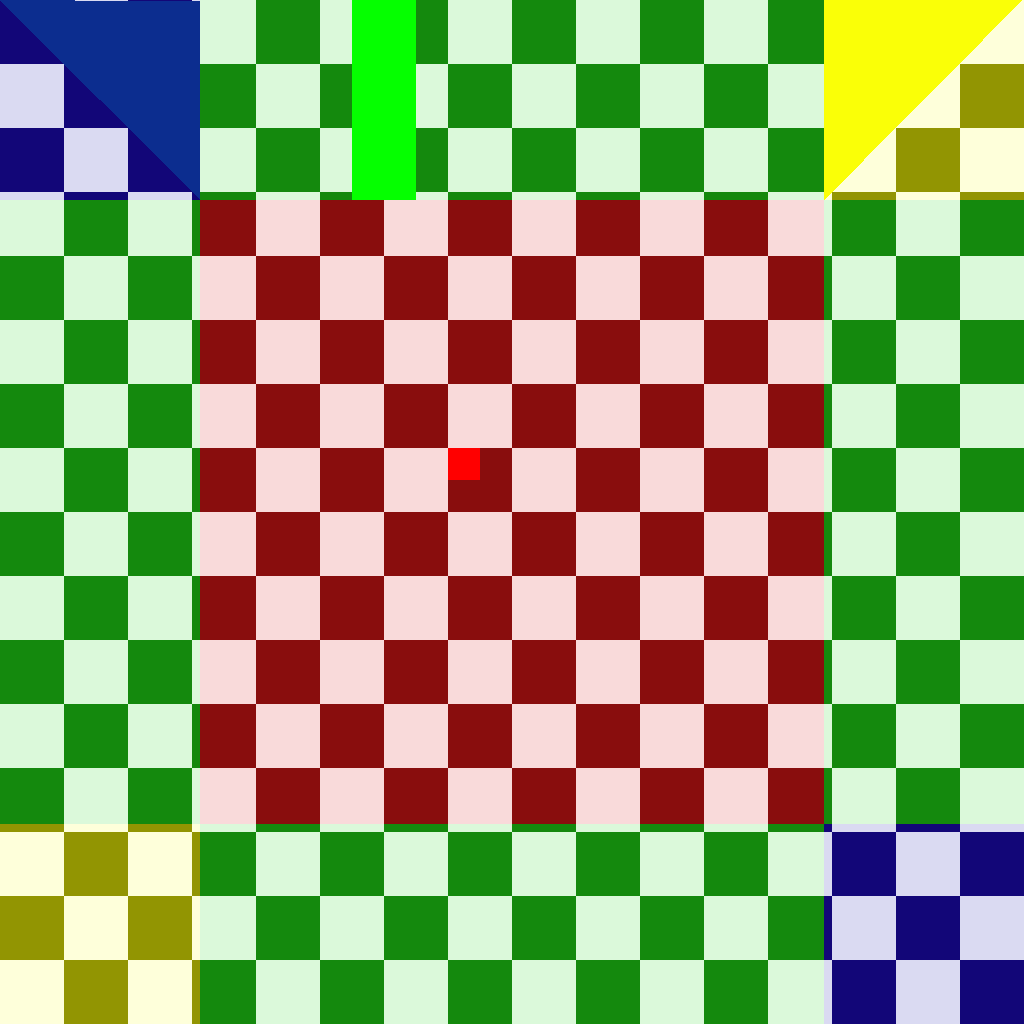
\includegraphics[width=150pt]{res/stencil_colored_with_prec}
	\caption{Colored 1024 x 1024 pattern assumming $k = 200$. Areas that need to be precomputed are opaque.}
	\label{fig:board}
	\end{center}
	\vspace{-0.3in}
\end{figure}

The blue corners can only be reused for the yellow corners
if they share the same colored tile (black or white) in the most outer part of the edge. This is only the
case if ($nx + ny) \equiv_{128} 0$

If either $nx \not\equiv_{64} 0$ or $ny \not\equiv_{64}0$, the right border or lower border,
respectively, and all corners need to be computed seperatly.
For all corners except the top-left one,
a whole square needs be computed instead of a triangle, because of the lack of diagonal symmetry.  
This leads to the number of points to be stenciled in Table~\ref{tab:numstencil}. Note that
in the last row of the table, only the worst case is specified, as the optimised program
tries to find further symmetries (e.g. between the right and lower border).

Because the number of points to be stenciled lies in $\Theta(k^2)$, the number of floating-point
operations lies in $\Theta(k^3)$ and is therefore asymptotically independent of the dimensions of the image. That also explains the small time differences between different sizes in Table~\ref{tab:prec} with precomputation compared to the bigger differences without.
If this optimisation does not decrease the number of points to be stenciled, the program falls back to stenciling the whole field.

\begin{table}[ht]
	\caption{Avg. number of points to be stenciled ($k' = 1.5k+0.5$)}
	\begin{tabular}{c c}
		variables & number of points\\
		\hline
		$\scriptstyle nx,ny \equiv_{64}0,(nx+ny) \equiv_{128}0$ & $ \frac{k'(k'+ 1)}{2} + 64k' + 32^{2}$\\
		$\scriptstyle nx,ny \equiv_{64}0,(nx+ny) \not\equiv_{128}0$ & $ k'(k'+1) + 64k' + 32^{2}$\\
		$\scriptstyle nx \not\equiv_{64}0 \lor \scriptstyle ny \not\equiv_{64}0$ & $ 3k'^{2} + \frac{k'(k'+1)}{2} + 3 * 64k' + 32^{2}$\\
	\end{tabular}
	\label{tab:numstencil}
\end{table}


\begin{table}[ht]
	\caption{Final version with and without precomputation ($k=200$, $\mu = \frac{\#points\ stenciled\ orig.}{\#points\ stenciled\ final\ }$).}
	\begin{tabular}{c c c c c}
		image size    & w.o. pre. & w. pre. & speedup & $\mu$  \\
		\hline
		1024 x 1024 & 0.0983s  & 0.0163s & 6.03 & 9.46\\
		4096 x 4096 & 3.235s  & 0.0269s & 120.26 & 152.34\\
		8000 x 8000 & 13.354s & 0.0451s  & 298.1 & 976.26\\
	\end{tabular}
	\label{tab:prec}
\end{table}


\section*{Memory Access and Vectorisation}
The original stencil code has many problems regarding its memory access patterns.
First of all, the outer loop operates on the rows and the inner loop on the columns.
This lead to a spray-like access patterns as the image is saved column-wise, which means
that two points on the same row are far away from each other.
To fix that problem I rearranged the image to be saved row-wise instead. It feels more
natural and allows better caching and access prediction.

\begin{table}[ht]
	\caption{Original version with row-wise compared to column-wise layout ($k=200$, \textit{gcc -O0}, average out of 10).}
	\begin{tabular}{c c c c}
  		 image size  & col-wise  & row-wise    & speedup  \\
		 \hline
		 1024 x 1024 & 5.908341s & 4.5175605s  &  1.308   \\
		 4096 x 4096 & 130.1964s & 73.140382s  &  1.78    \\
		 8000 x 8000 & 561.1181s & 275.47884s  &  2.037   \\
	\end{tabular}
	\label{tab:row}
\end{table}

%\textbf{Roofline Model}


%- Alignment
%- \_\_builtin\_assume\_aligned
%- speedups
%- replace memcpy with for loops
The processor found on the \textit{bc4} is the \textit{Intel Xeon E5-2680 v4} introduced in 2016.
According to the official intel spreadsheet\footnote{\url{https://ark.intel.com/content/www/us/en/ark/products/91754/intel-xeon-processor-e5-2680-v4-35m-cache-2-40-ghz.html}},
it supports the \textit{AVX2} instruction set extension, which allows vector operations on up to 256 bits.
When using the right flags (\texttt{icc -xCORE-AVX2 -simd}) the compiler already starts to vectorize many operations in the original version.
This can be observed by looking at the disassembly which now contains \textit{AVX2} instructions
at the stencil symbol (e.g. \texttt{vmulsd, vmovsd}); but also using the \textit{Intel Advisor}\footnote{\url{https://software.intel.com/en-us/advisor}} tool,
which asserts that 96.3\% of the time in the stencil function is spent in vectorized loops (1024 x 1024 case).

After applying the row-wise layout, this number grows to 98.8\%. This smaller difference
can also be observed when comparing the speedup between versions. Comparing this speedup with the one \textit{gcc} produced we can assume
that the \textit{icc}-Compiler with the right flags already optimised the row/column layoutin a good way.

\begin{table}[ht]
	\caption{Layout optimisation compared to vectorisation added ($k=200$).}
	\begin{tabular}{c c c c}
  		 image size  & layout  & vectorize    & speedup  \\
		 \hline
		 1024 x 1024 &  &  &     \\
		 4096 x 4096 &  &  &     \\
		 8000 x 8000 &  &  &     \\
	\end{tabular}
	\label{tab:flags}
\end{table}


- row caching, no temp field
- first cols, than rows
- padding, assume\_aligned, memalign, mmap, retrict

\section*{Other Improvements}

- compiler flags
- failed attempts

\section*{Further possible Improvements}

% -------------------------------------------------------------------------------
\section*{Conclusion}
% -------------------------------------------------------------------------------


\bibliographystyle{plain}
\bibliography{lit}

\end{document}
